\documentclass[12pt]{article}
\usepackage[letterpaper]{geometry}
\usepackage{amsmath, amsthm, amssymb, amsfonts}
\usepackage{graphicx}
\usepackage{titling}
\newcommand{\subtitle}[1]{%
  \posttitle{%
    \par\end{center}
    \begin{center}\large#1\end{center}
    \vskip0.5em}%
}
\title{CSE 150 - Operating Systems \\ Documentation \#1}
\subtitle{Spring 2018 - Lab 04 - Group 1}
\author{Avery Berchek, Aleksandr Brodskiy, David Cabral, Christopher DeSoto,\\Adiam G-Egzabher, Nanditha Embar, Christian Vernikoff}
\begin{document}
\maketitle
{\setlength{\parindent}{0cm}
\textbf{Outline}
\begin{enumerate}  
\item Documentation
\item Design Decisions
\item Testing/QA
\item Design Questions
\item Team Member Work-Log
\item Conclusion\\\\\\\\\\\\\\\\
\end{enumerate} 
}
{\setlength{\parindent}{0cm}
\textbf{Documentation}\\
\begin{center}Task 1\end{center}
The implementation of the \textsc{join} function is of significant relevance in building a multi$-$thread system due to the fact that the joining of multiple threads relies on the preoccupation of the system's resources on the execution of a currently processing thread. In essence a full and complete functional implementation of the \textsc{join} function would mitigate, not ameliorate, the problematic occurence of priority inversion. The logic required for the sucessfully joining of two or more threads is defined in the \textsc{KThread.java} class which makes use of system interrupts as follows: \begin{center}\textsc{boolean machine\underline{\hspace{.3cm}}start\underline{\hspace{.3cm}}status = Machine.interrupt().disabled(); \\ Machine.interrupt().disable();}\end{center} In this manner the current state of the machine is stored before any actions are performed. As such, threads would not be waiting endlessly even if there were to be an unexpected abnormal termination. This functionality is actual achieved through an algorithmic set$-$up of the \textsc{join} function which is implemented upon conditional checks, \textsc{if}$-$statements, and an iterative procedure, \textsc{while}$-$loop, in order to parse through a priority queue. This logic allows the NachOS machine to terminate a thread upon the invocation of the \textsc{join} functionality. For instance, given two threads; thread\underline{\hspace{.3cm}}1 \& thread\underline{\hspace{.3cm}}2, the execution of the latter thread would be paused until execution of the former is fully complete, respectively. In this manner, the logic behind the implementation of the \textsc{join} function is demonstrated in the following pseudo-code:\\
\\ 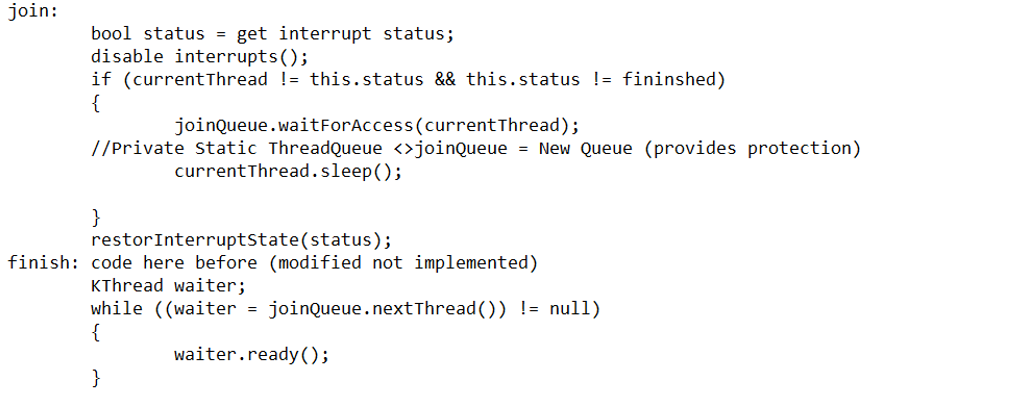
\includegraphics[width=180mm]{pic1.png} \\ 
 \begin{center}Task 2\end{center} 
The actualization of a direct automation functionality for condition variables was implemented in the \textsc{Condition.java} and \textsc{Condition2.java} classes. Within this implementation  the \textsc{wakeall} function, although allows the saving capability in regards to competing resources, is mainly used for synchronization of them. In essence, this design is analogous to the \textit{Token Ring} network protocol, in which the \textit{condition} mirros the utilization of the \textit{token} itself and therefore enables an interface to wake other participants in order to provide a method for their respective synchronization. In this manner establishing a systematic hierarchical automaticity. The pseudo-code demonstrates the functions invoked to achieve this implementation:
\begin{center} 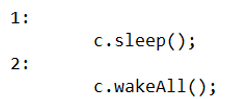
\includegraphics[width=40mm]{pic2.png} \end{center}
In this manner the \textsc{wake} and \textsc{wakealls}functions were composed as follows:
\begin{center}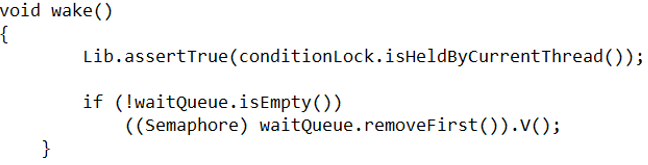
\includegraphics[width=120mm]{pic6.png}\end{center}
Within this implementation it is observable that the priority queue was controlled with a \textit{while}$-$loop condition to check for emptiness of the \textsc{waitQueue} of semaphores.
\begin{center}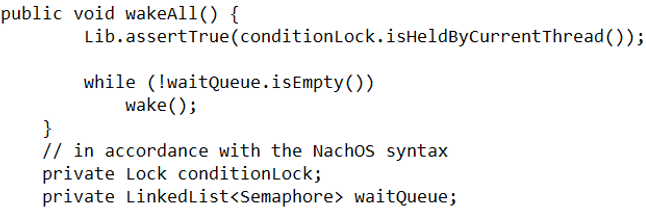
\includegraphics[width=120mm]{pic7.png}\end{center}
Although the direct application of \textit{Semaphores} was avoided in the aforementioned design, it is paramount to this documentation and more importantly, to the concerns addressed in the \textbf{Design Decisions} section, to emphasize the fact that the functions \textit{P} and \textit{V} from the \textsc{Semaphore} class were mapped to the \textsc{lock.java} class in the interest of utilizing the \textsc{acquire} and \textsc{release} functions respectively.
\\\\  
\begin{center}Task III\end{center}
The consummation of the \textsc{alarm.java} class was achieved by including a \textsc{waituntil} functionality to the previously established multi$-$threading system in order to suspend the execution of a thread prior to the completion of a thread released from the priority queue. The value of such a function essentially resides in the dependence real$-$time thread operations have on hierarchical administration. The implementation involved  utilization of the built$-$in \textsc{java} priority queue class under the pretense that the timer executes only once every 500 clock ticks. In this manner, the current system time was made retrievable through the \textsc{machine.timer} and \textsc{.gettime} function calls repectively. The following pseudo$-$code demonstrates the algorithmic structure of the logic.
\begin{center} 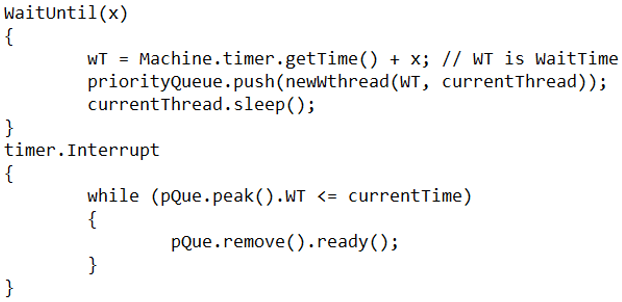
\includegraphics[width=120mm]{pic3.png} \end{center} 
As observable in the pseudo$-$code, the time elapsed can be calculated by adding the function argument denoted by the variable \textsc{x} to \textsc{Machine.timer.getTime()}: \begin{center} \textsc{waittime} = \textsc{Machine.timer.getTime()} + \textsc{x}; \end{center}Where \textsc{x} represents the number of ticks. Consequently, resolution can be achieved by applying a sorted priority queue based on time and storing the thread as well as the corresponding time in the queue. Basically, this resolution allows for any number of threads to invoke the \textsc{waituntil} function and be suspended from execution at any particular time.
\begin{center}Task IV\end{center}
In order to fully and completely implement the synchronous sending and receiving of one word messages the \textsc{speak} and \textsc{listen} functions were designed with the intent of ensuring that the proper speaker returns an acknowledgment or a desired reciprocated action per consumed word. For instance, given two communicators; T\underline{\hspace{.3cm}}1 and T\underline{\hspace{.3cm}}2, if T\underline{\hspace{.3cm}}1 speaks 1 and T\underline{\hspace{.3cm}}2 speaks 2 then T\underline{\hspace{.3cm}}1 should return when 1 is consumed by the \textsc{listen}ers and T\underline{\hspace{.3cm}}2 should return when 2 is consumed. This intention is demonstrated in the following pseudo$-$code: \begin{center} 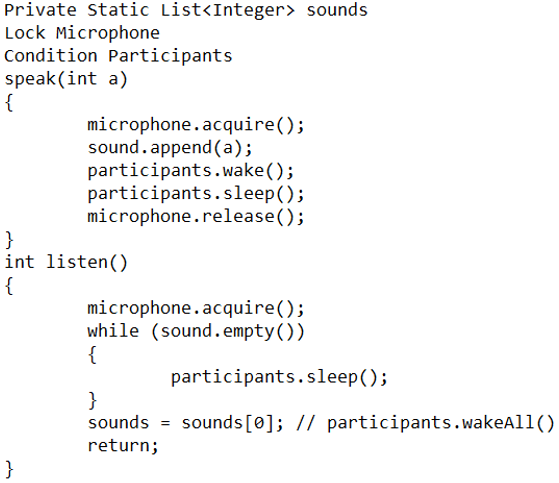
\includegraphics[width=100mm]{pic4.png} \end{center}
As perceivable, reciprocation was achieved by utilization of the \textsc{lock} feature to delineate between threads that are speaking in order to transition the remainder of the threads into the sleep state. This property is true of both the \textsc{speak} and \textsc{listen} functions as they both utilize an iterative procedure, \textsc{while}$-$loop, in order to establish a sleeping state while the systems remains idle until a thread speaks. This implementation, in essence, allows for potential multiple speakers to broadcast the same word without contingency.
\begin{center} Task V\end{center}
The implementation of priority scheduling in the \textsc{PriorityScheduler.java} class was achieved through the application of a \textsc{ThreadQueue} \textit{sub$-$class}. In this manner the initially proposed pseudo$-$code was designed with the intention of utilizing the following abstractions:\begin{center}\textsc{
ThreadedKernel.scheduler\\nachos.threads.RoundRobinScheduler\\nachos.threads.PriorityScheduler
}\end{center}
as a priority value for the \textsc{threadstate.java} class. Essentially this would invoke the corresponding priority value as a means of organizing threads in a hierarchical manner to deduce the order of execution. Keeping track of necessary elements requires the addition of a new data structure, \textit{i}\textbf{.}\textit{e}\textbf{.} treeset, in the priority queue, a hash set and a priority queue within the thread state. The treeset structure inside the priority queue class is intended to hold all the threads that will be managed within the priority queue. The hash set structure in the thread state class is meant to hold all the queues that are owned by the thread to be able to calculate effective priority. The extra priority queue within the thread state class is meant to resemble the queue that the thread is currently waiting in. With these data structures, the developed algorithm becomes fully capable of correctly implementing the priority scheduler. Therefore, if there were to be multiple threads with identical priority values, this issue would be resolved with the utilization of the \textsc{nachos.threads.roundrobinscheduler} abstraction. In this manner, the logic behind the implementation of the aforementioned functionality is demonstrated in the following excerpt of pseudo-code:
\begin{center} 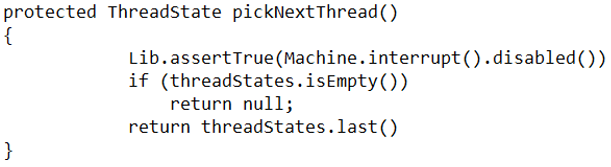
\includegraphics[width=102mm]{pic8.png} \end{center}
Additionally, the above outlined \textsc{NextThread} and two synthesized functions,
\textsc{update} and \textsc{recalculateThreadScheduling} were defined as follows:\\
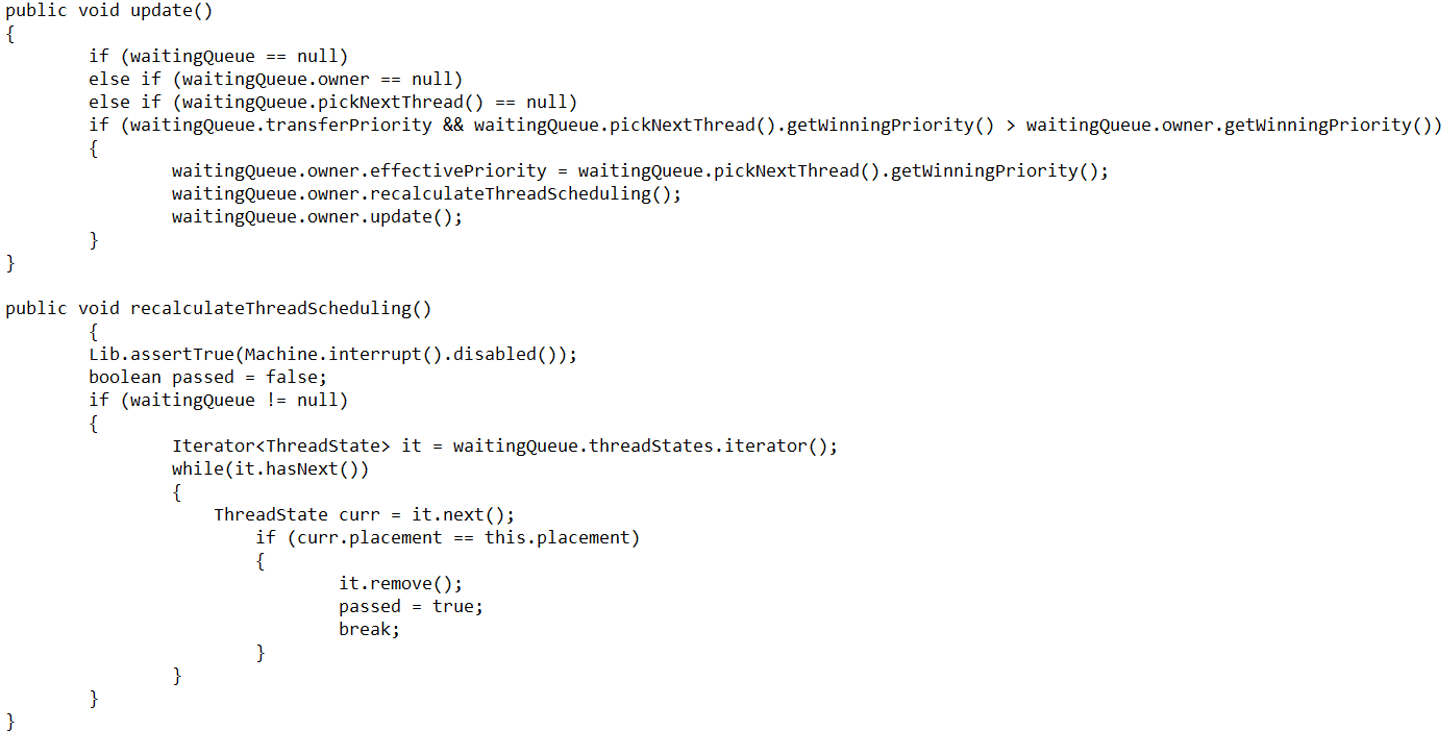
\includegraphics[width=180mm]{pic9.png}\\
By obersvation it is concludable that in order to be able to implement the correct ordering of threads within the queues, a comparator is implemented that would take into account a thread's priority, time put in the queue and another value which is labeled as placement in the submitted code. This algorithmic functionality would be used for the case in which a thread has the same time and same priority. The placement value would essentially implement the \textsc{nachos.threads.roundrobinscheduler} when time and priority couldn't be used. 
\begin{center}Task VI\end{center}
In order to develop and implement a complete and efficient solution to the Oahu$\longrightarrow$Molokai problem, a proposed implementation would invoke prioritizing children moving from Oahu to Molokai. As such, \textsc{child}ren would occupy Molokai before the \textsc{adult}s would and simultaneously function as pilots for the transmitting boat back to Oahu such that the \textsc{adult}s can then pilot themselves in the interest of prohibiting \textsc{child}ren from commuting with \textsc{adult}s on the boat. In this manner unlike \textsc{child}ren, \textsc{adult}s would refrain from returing to Oahu. Due to the fact that there are at least two \textsc{child}ren, there will be at least one child waiting on Molokai who will consequently be able to function as a pilot to bring the boat back to its original state in Oahu, where this process would perpetuate. This method of \textsc{child}ren interchangeably switching boat rides with adults will ensure that the adults will eventually occupy Molokai irrespective of the number of \textsc{adult}s in relation to the \textsc{child}ren. The initializer for the \textsc{child}ren and \textsc{adult} threads is the \textsc{begin} function which is implemented as follows:
\begin{center} 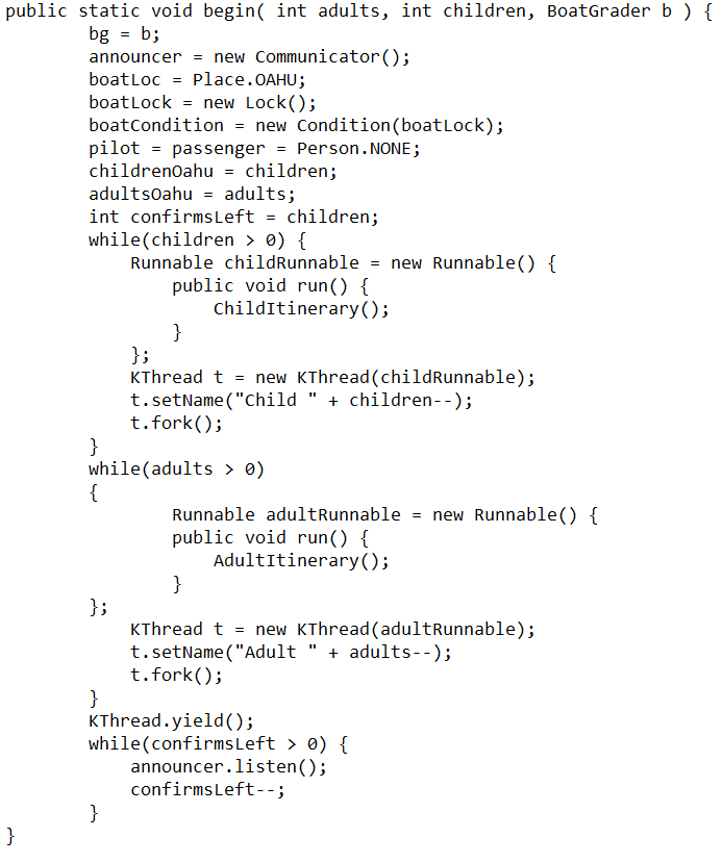
\includegraphics[width=102mm]{pic5.png} \end{center}
This function terminates once all \textsc{child}ren singal transfer completion. In this manner the \textsc{child} and \textsc{adult} itineraries are as follows: 
\begin{center} 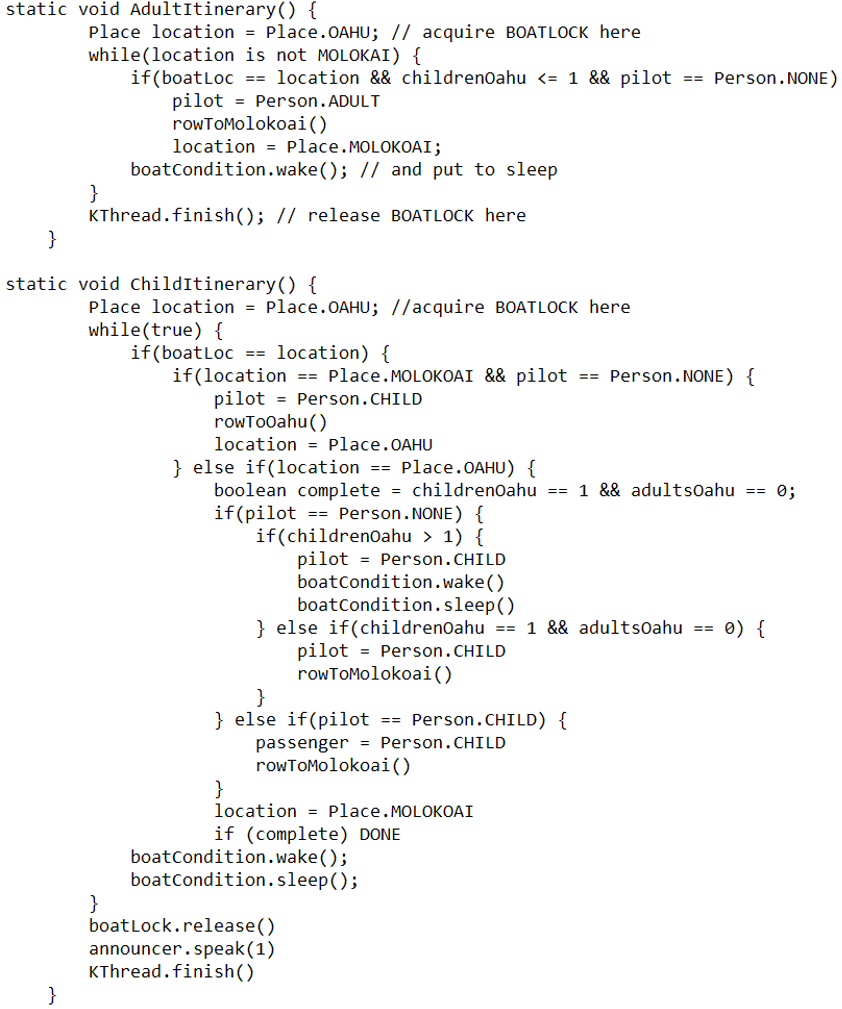
\includegraphics[width=150mm]{pic10.png} \end{center} As such, these functions consummate the breadth of the logical infrastructure developed for the \textsc{Boat.java} class\\.
}
{\setlength{\parindent}{0cm}
\textbf{Design Decisions} \\
The primary factors of significant importance to the design considerations for the development of a thread system were the scalability, robustness, and efficiency of the system in accordance with the resources associated with its support. In this manner the utilization of data structures, primitive types included, such as priority queues was preeminently regnant to the functionality of the objects defined. For example priority queues were utilized for the established \textsc{condition varibles}, \textsc{alarm} objects, as well as the priorities associated with various threads. This dependence on priority queues was paramount to the efficiency of the system. Likewise, an important design decision was the integration of the \textsc{release} and \textsc{acquire} functionalities from the \textsc{semaphore.java} class which were defined there as the \textit{P} and \textit{V} functions. This integration was achieved by transcribing the functions and accounting for the variable and object discrepancies between the two classes. This design resulted in the ability to utilize the \textsc{release} and \textsc{acquire} functions in order to possess and control a lock with a thread in a non$-$dormant state. Another design decision formed during the implementation of scheduling in the \textsc{PriorityScheduler.java} class was the addition of the following functions: \begin{center}\textsc{update();\\	recalculateThreadScheduling()}\end{center} These functions provide abstractions to maintain threads and their corresponding data structures. The \textsc{update} function is called whenever a thread changes it's priority or effective priority so as to be able to affect the effective priorities of the thread that own the queue of where one of their thread's priorities changed; whether it be effective or regular priority. For the purpose of affecting structures of priority queues, the \textsc{update} function is called recursively by traversing through the owners of queues and affecting the owners with the potentially changed priority values. Likewise the \textsc{recalculateThreadScheduling} function is a function that is made to keep the data structures updated as their dynamic values and elements change throughout run$-$time. The underlining discrepancy between these two functions is that the latter is meant to deal with the specific data structure being used by utilizng \textit{treeset} because \textit{treeset} doesn't automatically reorganize the set when one element changes so this function essentially removes the element then adds it again so that the data structure can be in the correct arrangement.\\These design decision provided for the redundancy and reusability of the code and as such reduced the necessity of pair programming practices for the purposes of code reviews as the reusability of code ensured proper functionality.\\\\ 
}
{\setlength{\parindent}{0cm}
\textbf{Testing/QA} \begin{center}Task I\end{center}
Testing the validity of the \textsc{KThread.join()} implementation was performed with multiple threads in the following arrangements; an even number and an odd number of threads. In this manner, the former arrangement was set$-$up with testing four threads where three of them join to the first. As such another test was executed in which eight threads were set$-$up where three threads join one and another three can join to another thread. These tests allowed to determine whether or not the \textsc{join} function properly does what is required in accordance with the design specifications. The latter arrangement however, sets$-$up a test in which three threads are utilizied to check if two would join to one. In order to test to check if a thread doesn’t join, nine threads are utilizied; while seven of them join to one thread leaving a single thread without the ability to join to another one. Therefore these two arrangements determine the functionality of the \textsc{join} function by testing how even and odd number of threads work with just one single join. In regards to edge cases however, testing for robustness and scalability was achieved by testing, incrementally, the number of threads being used. 
\begin{center}Task II\end{center}
	For the \textsc{Condition.java} and \textsc{Condition2.java} condition variables classes testing was set$-$up and executed in the following manner; to interrupt enable and to disable in the interest of ensuring that there is no waking up waiting threads. In essence, the control check that the queue storing threads is not empty in conjunction with the interrupt function being is disabled by default served as the predominant \textit{sanity check}.\\ To stress test these different conditions, a \textsc{lock} variable may be synthesized to make sure that while a thread is invoked the \textsc{lock} remains \textsc{lock}ed and then put to sleep for each thread inside the {lock}. After the threads have completed their utilization of the \textsc{lock}, the \textsc{wake} function may be invoked to wake the first waiting thread in the wait queue.
\begin{center}Task III\end{center}
The \textsc{Alarm.java} test cases were primarily executed with different times for the \textsc{waitUntil} function argument variable. Therefore forming a methodology to account for and essentially test for different timer conditions. These varied tests were performed iteratively to account for as many conditions as possible. In addition to these trivial test case, the corner cases were performed as follows; a wait time of 0 as well as an arbitrarily long wait time of 1000000 were hard coded. This strategy allowed stress testing the implementation in extreme cases to determine robustness and scalability.
\begin{center}Task IV\end{center}
In \textsc{Communicator}, the main tests needed to be run to test how the implementation handled multiple \textsc{listen}ers/\textsc{speak}ers were set$-$up with two discrepant scenarios. These scenarios would naturally be the most demanding and stressful, and so would reveal any hidden errors that might arise under similar, or less stressful loads.\\
The first part of the test loads up the many \textsc{listen}ers test, and checks if the \textsc{listen}ers hear the single \textsc{speak}er. The second test creates many threads and designates them to \textsc{speak} to only a sole \textsc{listen}er. It then checks if the \textsc{listen}er heard the spoken word.
\begin{center}Task V\end{center}
For general testing, there are two situations that were tested to check for working functionality. They were testing for when priority donation was being used and for when it wasn’t. Some estimated corner case testing was also used such as making sure thread states were changed correctly for when a thread lost ownership of a priority queue. \\ Testing without priority donation was kept simple in the sense that making sure that priority wasn’t donated to the owner of the queue. For future test cases, going to mix in queues that have transfer priority and those that don’t, that share a common owner to make sure that the owner’s effective priority considers the relevant queues priorities. \\Testing with priority donation involved making three queues and filling them each with threads of various priorities. One thread queue would be filled with the highest priority out of the three queues as so to be able to see that the priority scheduler was able to assign the correct highest priority to the owner of all three thread queues. Thread priorities would be changed through out the program to be able to see that changes were correctly updated throughout the thread queue structure. \\	Some corner case scenarios that were considered that weren’t as general as the previous testing was checking the values of thread states in scenarios such as when a thread would lose ownership of a queue when next thread would be called. Reasoning for checking this was because when a thread loses ownership of a queue, then that thread’s effective priority has a possibility of changing to something lower or staying the same. 
\begin{center}Task VI\end{center} 
Although there had been some unsuspected issues with the initializers of the \textsc{child} and \textsc{adult} objects in the \textsc{Boat.java} class, these issues had been mitigated simply with the //\textit{commenting} out of the initializer statements. \\The testing process was relatively straight$-$forward in the sense that a plethora of stress tests were performed all with various, arbitrary combinations of \textsc{child}ren and \textsc{adult}s. Consequently, the corner cases were performed in which there no \textsc{adult}s or \textsc{child}ren respectively, per test.\\\\
}
{\setlength{\parindent}{0cm}
\textbf{Design Questions} \\
\\ Why is it fortunate that we did not ask you to implement priority donation for \textsc{semaphores}?
\\ \textit{It is fortunate because each time a thread acquires a lock or calls the \textsc{join} function, the allocator of the resource is acknowledged which enables the further donation of resources in priority to the single, aforementioned, allocator resource. This is true if a thread with a higher$-$priority rating remains in an idle state however if this functionality were to be implemented with semaphores, it would not be fully and completely utilizable because the last thread to \textsc{acquire} the semaphore will not necessarily be thread of lower/lowest$-$priority. In this manner the implementation would need amends maintain all threads that are currently utilizing the semaphore.} \\\\ A student proposes to solve the boats problem by use of a counter, \textit{AdultsOnOahu}. Since this number isn't known initially, it will be started at zero, and incremented by each adult thread before they do anything else. Is this solution likely to work? Why or why not? \\ \textit{This solution will most likely fail due to the fact that would be no metric such as to delineate and provide the prescription for everyone who would, potentially, increment the counter pro$-$actively.}
\\\\\\\\\\\\\\\\\\\\\\
}
{\setlength{\parindent}{0cm}
\textbf{Team Member Work-Log}\\ \\
\textbf{\begin{center}\underline{Avery Berchek}\\DevOps Engineer\end{center}} 
\begin{itemize}
\item{Designed and outlined the pseudo$-$code for Task I, II, \& IV}
\item Outlined and participated in the design process associated with Tasks I, II, III, IV, V, \& VI
\item{Implemented the algorithmic functionality for Tasks I, II, IV, \& VI}
\item{Primarily responsible for implementation of corner$-$case test cases}
\item{Conducted and performed code reviews}
\item{Performed optimizations and ensured the efficiency of the data structures utilized in the source code}
\end{itemize}
\textbf{\begin{center}\underline{Aleksandr Brodskiy}\\Project Manager\end{center}}  
\begin{itemize} 
\item Organized the \textit{sprints} and weekly meetings in accordance with the \textit{Agile/Scrum} project management methodology.
\item Delegated tasks and assigned roles for the Engineering Team as well as conducted the code reviews
\item Created and formatted the Design Documentation
\item Managed all progress and operations of the Engineering Team in order to provide an efficient, robust, and optimal solution for a timely and submission. \\ \\
\end{itemize}
\textbf{\begin{center}\underline{David Cabral}\\Design Engineer\end{center}} 
\begin{itemize}
\item Designed and outlined the pseudo$-$code for Task V
\item Implemented the algorithmic functionality for Tasks V \& VI
\item Provided insight and proposed solution for \textit{Priority Scheduling}
\item Proposed solution and outlined source code structure for Task VI
\end{itemize}
\textbf{\begin{center}\underline{Christopher DeSoto}\\Principal Engineer\end{center}}
\begin{itemize} 
\item Set$-$up the integrated development environment for the entire Engineering Team.
\item Outlined and participated in the design process associated with Tasks I, II, III, IV, V, \& VI
\item Integrated source code from the \textit{development phase} to the \textit{testing phase} to the \textit{completed phase} to ensure the validity of the solution and provide a general framework for the debugging and testing process for the QA and Software Engineers. \\ \\
\end{itemize}
\textbf{\begin{center}\underline{Adiam G-Egzabher}\\Systems Engineer\end{center}} 
\begin{itemize}
\item Outlined and participated in the pseudo$-$code development associated with Task VI
\item Participated in the design process and testing/QA phase for Tasks IV, V, \& VI
\end{itemize}
\textbf{\begin{center}\underline{Nanditha Embar}\\QA Engineer\end{center}} 
\begin{itemize}
\item Ensured functionality of all features 
\item Ensured the highest quality attainable with the time and resources provided for submitted source code
\item Participated in the design process and testing/QA phase for Tasks I, II, \& III
\end{itemize}
\textbf{\begin{center}\underline{Christian Vernikoff}\\Software Engineer\end{center}} 
\begin{itemize}
\item{Designed and outlined the pseudo$-$code for Task I \& III}
\item{Implemented the algorithmic functionality for Tasks I, III, \& VI}
\item Outlined and participated in the design process associated with Tasks I, II, III, IV, V, \& VI
\item{Debugged and performed all necessary tests for Task I \& III}
\end{itemize}
}
{\setlength{\parindent}{0cm}
\textbf{\\\\\\Conclusion}\\ \\
As a result of completing an efficient and optimized solution to the aforementioned tasks, a foundational component of an operating system, a thread structure, was formed. This thread system will be utilized in the formation of a operating system scheduler for the development of more advanced multi$-$functional operating system features. 
\end{document} 
